\documentclass{beamer}	
\usecolortheme{default}

\setbeamertemplate{caption}{\raggedright\insertcaption\par}

\usepackage{tabularx}
\usepackage{booktabs}
\usepackage{multirow}
\newcolumntype{C}{>{\centering\arraybackslash}X}
\usepackage{proof}
\usepackage{amsmath}
\usepackage{wasysym}
\usepackage{tikz}
\usetikzlibrary{arrows.meta,positioning,matrix}
\usetikzlibrary{shapes.multipart, calc}
\usepackage{tikz-qtree}
\usepackage{soul}
\usepackage{mathtools}

\newcommand{\term}[1]{\ensuremath{\mathtt{#1}}}
\newcommand{\li}{\!\multimap\!}
\newcommand{\lotimes}{\!\otimes\!}
\newcommand{\loplus}{\!\oplus\!}
\newcommand{\lin}[1]{\langle#1\rangle}
\newcommand{\lint}[1]{[#1]}
\newcommand{\cat}[1]{\footnotesize \textsc{#1}}	
\newcommand{\W}[1]{\scriptsize #1}
\newcommand{\etext}[1]{\scriptsize {\textit{#1}}}
\newcommand{\smain}{\cat{S}$_{\text{main}}$}
\newcommand{\ssub}{\cat{S}$_{\text{sub}}$}
\newcommand{\type}[2]{\scriptsize\ensuremath{\textcolor{#2}{#1}}}
\newcommand{\red}[1]{\textcolor{red}{{}_#1}}
\newcommand{\dia}[1]{\overset{#1}{\Diamond}}
\newcommand{\bx}[1]{\overset{#1}{\Box}}

\title{Data-driven logic}
\author{K. Kogkalidis}
\institute{Logic \& Language 2020}

\begin{document}

\begin{frame}{..continuing}
\small
The agenda:
\begin{itemize}
	\item[$\lambda$] \textcolor{gray}{Choosing the logic}
	\item[$\lambda$] \textcolor{gray}{Making a dataset: proofs and lexical type assignments}
	\item[$\lambda$] \alert{Learning the type assignment process}
	\item[$\lambda$] \alert{Navigating the proof space}
	\item[$\lambda$] \textcolor{gray}{Syntax-aware \& type-correct text representations}
\end{itemize}
\end{frame}

\begin{frame}{Lexical type ambiguity}
	\small
	
	\alt<3>{
	\begin{figure}
		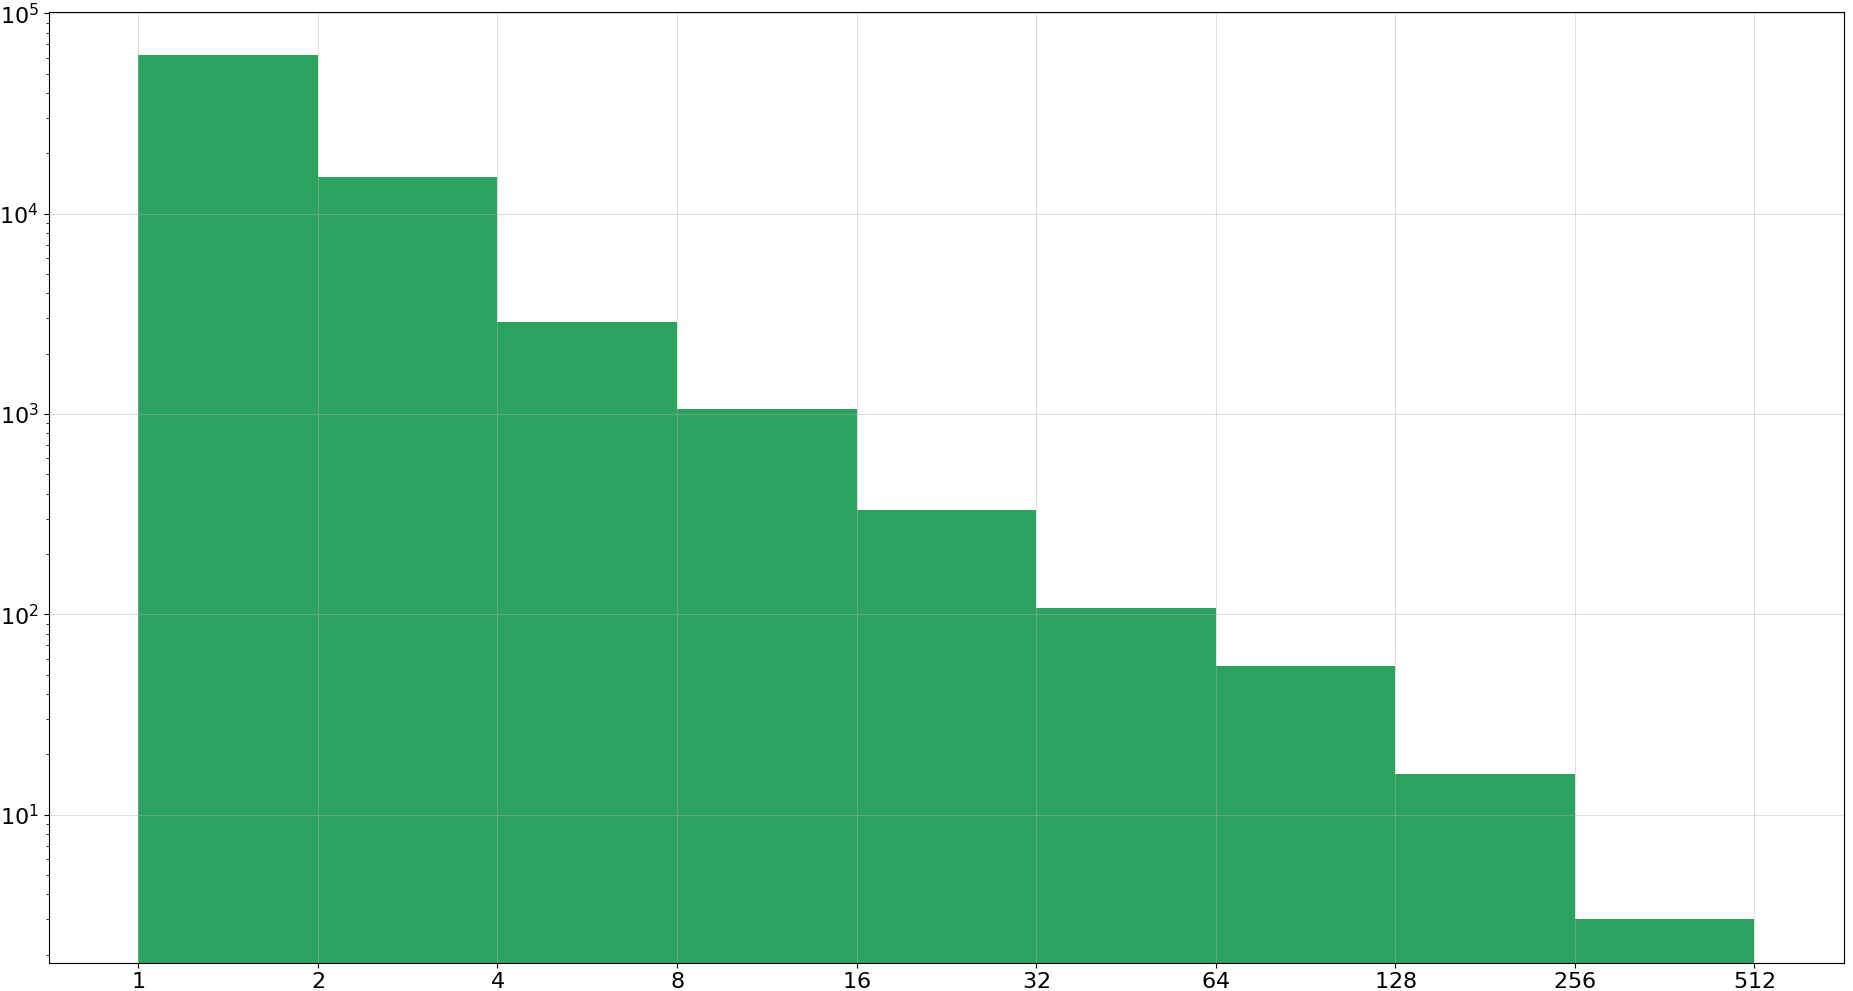
\includegraphics[width=0.99\textwidth]{oracle.png}
		\caption{\# types {\footnotesize(\textit{log2-transformed})} per word}
	\end{figure}
	}{
	\alt<2>{
		generally:
		\[
			w :: t_1 \& t_2 \& t_3 \& \dots \& t_n
		\]
		\vfill
			
		more refined grammar $\implies$ 
		\begin{itemize}
			\item[\frownie] harder lexical disambiguation (more $n$ per word)
			\item[\smiley]  easier parsing (\textit{if} one starts from correct type)
		\end{itemize}
	}{
	Type assignments are often \textit{ambiguous} and context-dependent:\vfill

	\begin{center}
	\begin{tabularx}{0.8\textwidth}{@{}rcl@{}}
	\multicolumn{3}{c}{\textbf{very realistic lexicon}}\\
	\toprule
	running :: 	& $\bx{mod}\left( np \li np \right)$ 					& \textit{running dog}\\
				& $inf$													& \textit{I like running}\\
	like		::	& $\dia{obj}np \li \dia{su}np \li s_m$					& \textit{ducks like seeds}\\
				& $\dia{obj}np \li \dia{su}pron \li s_m$					& \textit{I like ducks}\\
				& $\dia{obj}inf \li \dia{su}np \li s_m$					& \textit{ducks like swimming}\\
				& $\dia{obj}inf \li \dia{su}pron \li s_m$				& \textit{I like swimming}\\
				& $\dia{obj}np \li \bx{mod}\left( s_m \li s_m \right)$	& \textit{I swim like a duck}\\
				& \dots \\
	\end{tabularx}
	\end{center}
	}}
\end{frame}

\begin{frame}{Supertagging}
	\small
	
	\begin{block}{General idea}
		Given a sentence $w_1, w_2, \dots , w_n$\\
		\quad find the type sequence $t_1, t_2, \dots t_n$ that maximimizes
		\[
			p(t_1, t_2, \dots t_n | w_1, w_2, \dots w_n, \theta)
		\]
		where $\theta$ the trainable parameter space
	\end{block}
\end{frame}

\begin{frame}{Discriminative approach}
	\small
	
	\begin{block}{Markov assumption}
		\begin{align*}
			& p(t_1, t_2, \dots t_n | w_1, w_2, \dots w_n, \theta) \\
			\approx &
			\prod_{i=1}^{n} p(t_i | w_1, w_2, \dots w_n, \theta)
		\end{align*}
	\end{block}
	
	\begin{itemize}
		\item[\smiley] 			contextualized token classification						
		\item[\alert{\frownie}]	single answer
		\item[\alert{\frownie}]	sample sparsity
		\item[\alert{\frownie}]	closed codomain assumption
	\end{itemize}
\end{frame}

\begin{frame}{Generative approach}
	\small
	
	\begin{block}{\st{Markov assumption}}
		\begin{align*}
			& p(t_1, t_2, \dots t_n | w_1, w_2, \dots w_n, \theta) \\
			\approx &
			\prod_{i=1}^{n} p(t_i | t_1, t_2, \dots, t_{i-1}, w_1, w_2, \dots w_n, \theta)
		\end{align*}
	\end{block}
	
	\begin{itemize}
		\item[\smiley] 			seq2seq translation
		\item[\smiley]			many answers
		\item[\alert{\frownie}]	sample sparsity 
		\item[\alert{\frownie}]	closed codomain assumption
	\end{itemize}
\end{frame}

\begin{frame}{Generative approach: one more step}
	\small
	The type syntax: 
	\[
		cod(\mathcal{L}) := A \ | \ \dia{d} T \li T' \ | \ \bx{d}\left( T \li T' \right)
	\]
	corresponds to a \alert{simple cfg} (in prefix notation) with meta-rules:
		\begin{align*}
			S & \to A 				& & \forall A \in \mathcal{A}\\
			S & \to \dia{d} S \ S	& & \forall d \in \mathrm{comps} \\
			S & \to \bx{d} S \ S 	& & 	\forall d \in \mathrm{adjns}
		\end{align*}
	i.e. each type $t_i$ can be written as a sequence of primitive symbols $\vec{\sigma}$
	
	\pause
	\begin{align*}
			& p(t_1, t_2, \dots t_n | w_1, w_2, \dots w_n, \theta) \\
			\approx &
			\prod_{i=1}^{m} p(\sigma_i | \sigma_1, \sigma_2, \dots, \sigma_{i-1}, w_1, w_2, \dots w_n, \theta)
	\end{align*}
	
	\begin{itemize}
		\item[\smiley]			each type contains many subtypes (less sparsity)
		\item[\smiley]			any valid types can be inductively constructed (open codomain)
	\end{itemize}
\end{frame}

\begin{frame}{Some implementation notes}
	\small
	\alt<3->{just attention}{RNNs \visible<2->{/w attention}}
	\begin{itemize}
		\item \alt<2->{one vector per sequence element (lossless)}{single state compresses entire sentence (lossy)}
		\item \alt<3->{fully parallel training (fast)}{temporal dependence during training (slow)}
	\end{itemize}
	
	\visible<4->{
	\begin{block}{open questions}
		\begin{tabularx}{0.99\textwidth}{@{}lll@{}}
			? & explicit tree structure		& (tree-shaped decoders)\\
			? & decoding order				& (linear order vs. easy first)\\
			? & ultra-long types				&	(two-step decoding, generic vs. concrete instances)\\
			? & inference time delay			& (linearization via kernel methods)\\
			? & logical constraints		& (reinforcement learning)\\
		\end{tabularx}
	\end{block}
	}{}
\end{frame}

	\newcommand{\posimpl}{\overset{+}{\multimap}}
	\newcommand{\negimpl}{\overset{-}{\multimap}}
	\newcommand{\posat}[1]{\overset{+}{\proofspace#1}}
	\newcommand{\negat}[1]{\overset{-}{\proofspace#1}}
	\newcommand{\proofspace}{\vphantom{()}}
	
\begin{frame}{Proof Ambiguity}
	\small
	The type system (being non-directional) permits too many parses:
	\vfill
	
	\begin{minipage}{0.5\textwidth}
	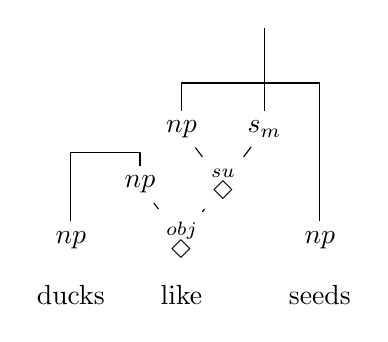
\begin{tikzpicture}[
	all node/.style={outer sep=0pt}
	]
		\node		(ducks)			at	(0,0)			{ducks};
		\node		(ducksnp)		at	(0,2em)			{$\posat{np}$};
		
		\node		(like)			at	(4em,0)			{like};
		\node		(likeobj)		at	(4em,2em)		{$\dia{obj}$};
		\node		(likenp1)		at 	(2.5em, 4em)		{$\negat{np}$};
		\node		(likesu)			at 	(5.5em, 4em)		{$\dia{su}$};
		\node		(likenp2)		at 	(4em, 6em)		{$\negat{np}$};
		\node		(likes)			at 	(7em, 6em)		{$\posat{s_m}$};
		\draw (likeobj) 	-- (likenp1);
		\draw (likeobj)	-- (likesu);
		\draw (likesu) 	-- (likenp2);
		\draw (likesu) 	-- (likes);
		\draw (likes)	-- ($(likes.north) + (0,3em)$);
		
		\node		(seeds)			at 	(9em, 0em)		{seeds};
		\node		(seedsnp)			at 	(9em, 2em)		{$\posat{np}$};
		
		\draw (ducksnp) -- ($(ducksnp.north) + (0,2.5em)$) -| ($(likenp1.north)$);
		\draw (seedsnp) -- ($(seedsnp.north) + (0,5em)$) -| ($(likenp2.north)$);
	\end{tikzpicture}	
	\centering
	\footnotesize
	\[
		\term{like\ (ducks)^{obj}\ (seeds)^{su}}
	\]
	\end{minipage}%
	\begin{minipage}{0.5\textwidth}
	\hfill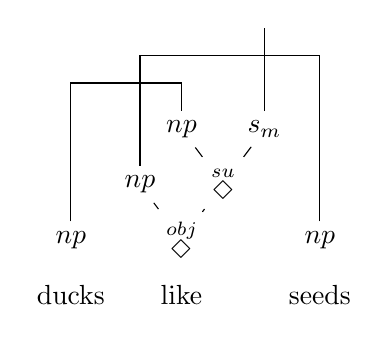
\begin{tikzpicture}
		\node		(ducks)			at	(0,0)			{ducks};
		\node		(ducksnp)		at	(0,2em)			{$\posat{np}$};
		
		\node		(like)			at	(4em,0)			{like};
		\node		(likeobj)		at	(4em,2em)		{$\dia{obj}$};
		\node		(likenp1)		at 	(2.5em, 4em)		{$\negat{np}$};
		\node		(likesu)			at 	(5.5em, 4em)		{$\dia{su}$};
		\node		(likenp2)		at 	(4em, 6em)		{$\negat{np}$};
		\node		(likes)			at 	(7em, 6em)		{$\posat{s_m}$};
		\draw (likeobj) 	-- (likenp1);
		\draw (likeobj)	-- (likesu);
		\draw (likesu) 	-- (likenp2);
		\draw (likesu) 	-- (likes);
		\draw (likes)	-- ($(likes.north) + (0,3em)$);
		
		\node		(seeds)			at 	(9em, 0em)		{seeds};
		\node		(seedsnp)		at 	(9em, 2em)		{$\posat{np}$};
		
		\draw (ducksnp) -- ($(ducksnp.north) + (0,5em)$) -| ($(likenp2.north)$);
		\draw (seedsnp) -- ($(seedsnp.north) + (0,6em)$) -| ($(likenp1.north)$);
	\end{tikzpicture}
	\centering
	\footnotesize
	\[
		\term{like\ (seeds)^{obj}\ (ducks)^{su}}
	\]
	\end{minipage}
	\vfill
	
	\pause
	\centering
	How can we select the correct one?
\end{frame}

\begin{frame}{Neural Proof Nets}
% pnet and tables
\scriptsize
\begin{center}
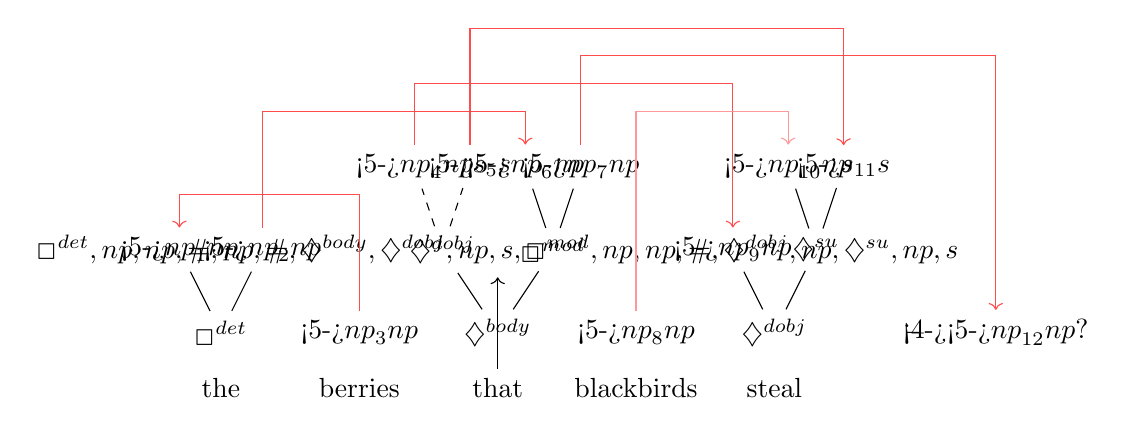
\begin{tikzpicture}
	% words
	\node (the)		at 	(0em, 0em)	{the};
	\node (berries)	at 	(5em, 0em)	{berries};
	\node (that)		at 	(10em, 0em)	{that};
	\node (birds) 	at 	(15em, 0em) 	{blackbirds};
	\node (steal)	at	(20em, 0em)	{steal};
	
	\visible<2-2>{
	\draw[->] (that) -- ($(10em, 4em)$);
	\node (test) 	at 	(10em, 5em) {
	$\Box^{det}, np, np, \#, np, \#, \diamondsuit^{body}, \diamondsuit^{dobj}, np, s, \Box^{mod}, np, np, \#, \diamondsuit^{dobj}, np, \diamondsuit^{su}, np, s$
	};
	}
	\visible<3->{
	% undecorated trees
	\node (thedet)		at	(0em, 2em)		{$\Box^{det}\proofspace$};
	\node (thenp1)		at	(-1.5em, 5em)	
		{\alt<5->{$\negat{np}_1$}{$\negat{np}$}};
	\node (thenp2)		at	(1.5em, 5em)		
		{\alt<5->{$\posat{np}_2$}{$\posat{np}$}};
	\node (berriesnp)	at 	(5em, 2em)		
		{\alt<5->{$\posat{np}_3$}{$\posat{np}$}};
	\node (thatbody)		at	(10em, 2em)		{$\diamondsuit^{body}\proofspace$};
	\node (thatobj)		at	(8em, 5em)		{$\diamondsuit^{dobj}\proofspace$};
	\node (thatobjnp)	at	(7em, 8em)		
		{\alt<5->{$\posat{np}_4$}{$\posat{np}$}};
	\node (thats)		at	(9em, 8em)		
		{\alt<5->{$\negat{s}_5$}{$\negat{s}$}};
	\node (thatmod)		at	(12em, 5em)		{$\Box^{mod}\proofspace$};
	\node (thatmodnp1)	at	(11em, 8em)		
		{\alt<5->{$\negat{np}_6$}{$\negat{np}$}};
	\node (thatmodnp2)	at	(13em, 8em)		
		{\alt<5->{$\posat{np}_7$}{$\posat{np}$}};
	\node (birdsnp)		at	(15em, 2em)		
		{\alt<5->{$\posat{np}_8$}{$\posat{np}$}};
	\node (stealobj)		at	(20em, 2em)		{$\diamondsuit^{dobj}\proofspace$};
	\node (stealobjnp)	at	(18.5em, 5em)	
		{\alt<5->{$\negat{np}_9$}{$\negat{np}$}};
	\node (stealsu)		at	(21.5em, 5em)	{$\diamondsuit^{su}\proofspace$};
	\node (stealsunp)	at  (20.5em, 8em)	
		{\alt<5->{$\negat{np}_{10}$}{$\negat{np}$}};
	\node (steals)		at 	(22.5em, 8em)	
		{\alt<5->{$\posat{s}_{11}$}{$\posat{s}$}};
	\node (vdash)		at 	(25em, 2em)		{$\vdash\proofspace$};
	\node (finalnp)		at 	(28em, 2em)		
		{\alt<4->{\alt<5->{$\negat{np}_{12}$}{$\negat{np}$}}{$?$}};
	
	% internal links
	\draw (thedet)   -- (thenp1);
	\draw (thedet)   -- (thenp2);
	\draw (stealobj) -- (stealobjnp);
	\draw (stealobj) -- (stealsu);
	\draw (stealsu)  -- (stealsunp);
	\draw (stealsu)  -- (steals);
	\draw (thatbody) -- (thatobj);
	\draw (thatobj)   edge[dashed] (thatobjnp);
	\draw (thatobj)   edge[dashed] (thats);
	\draw (thatmod)  -- (thatmodnp1);
	\draw (thatmod)  -- (thatmodnp2);
	\draw (thatbody) -- (thatmod);
	
	% axiom links
	\visible<8->{
	\draw[->, red!70] (berriesnp) -- ($(berriesnp) + (0em, 5em)$) -| (thenp1);
	\draw[->, red!70] (thenp2) -- ($(thenp2) + (0em, 5em)$) -| (thatmodnp1);
	\draw[->, red!70] (thatobjnp) -- ($(thatobjnp) + (0em,3em)$) -| (stealobjnp);
	\draw[->, red!70] (thats) -- ($(thats) + (0em, 5em)$) -| (steals);
	\draw[->, red!70] (thatmodnp2) -- ($(thatmodnp2) + (0em, 4em)$) -| (finalnp);
	\draw[->, red!40] (birdsnp) -- ($(birdsnp) + (0em, 8em)$) -| (stealsunp);
	}
	}
\end{tikzpicture}
\end{center}	
\vfill

\begin{minipage}[c]{0.75\textwidth}
\alt<2->{
\alt<3->
{
\alt<4->
{
\alt<5->
{
\alt<6->
{
\alt<7->
{7. train against ground-truth axiom links}
{6. discretize result with \textrm{Sinkhorn}}
}
{5. fill table with pair-wise agreement scores}
}
{4. index pos/neg occurrences and arrange in a table}
}
{3. find conclusion as the singleton $\mathcal{A}^+ - \mathcal{A}^-$}
}
{2. parse types to trees and assign polarity information}
}
{
1. pass the sentence through the supertagger
}
\end{minipage}%
\begin{minipage}[c]{0.25\textwidth}
\visible<5->{
		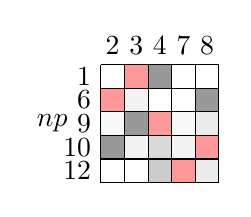
\begin{tikzpicture}[scale=.3]
		% matches
		\visible<6>{
		\fill[gray!60] (1, 4) rectangle +(1,1);
		\fill[gray!10] (1, 1) rectangle +(1,1);
		\fill[gray!20] (1, 2) rectangle +(1,1);
		\fill[gray!10] (1, 3) rectangle +(1,1);
		\fill[gray!80] (0, 3) rectangle +(1,1);
		\fill[gray!5] (0, 2) rectangle +(1,1);
		\fill[gray!5] (0, 1) rectangle +(1,1);
		\fill[gray!40] (2, 2) rectangle +(1,1);
		\fill[gray!30] (2, 1) rectangle +(1,1);
		\fill[gray!40] (2, 0) rectangle +(1,1);
		\fill[gray!10] (2, 4) rectangle +(1,1);
		\fill[gray!50] (4, 1) rectangle +(1,1);
		\fill[gray!15] (4, 2) rectangle +(1,1);
		\fill[gray!15] (4, 0) rectangle +(1,1);
		\fill[gray!20] (4, 3) rectangle +(1,1);
		\fill[gray!90] (3, 0) rectangle +(1,1);
		\fill[gray!10] (3, 1) rectangle +(1,1);
		\fill[gray!5] (3, 2) rectangle +(1,1);
		\fill[gray!5] (3, 0) rectangle +(1,1);
		}
		\visible<7->{
		\fill[black!40] (1, 2) rectangle +(1,1);
		\fill[black!40] (0, 1) rectangle +(1,1);
		\fill[black!40] (2, 4) rectangle +(1,1);
		\fill[black!40] (4, 3) rectangle +(1,1);
		\fill[black!40] (3, 0) rectangle +(1,1);
		}
		\visible<8->{
		\fill[red!40] (1, 4) rectangle +(1,1);
		\fill[red!40] (0, 3) rectangle +(1,1);
		\fill[red!40] (2, 2) rectangle +(1,1);
		\fill[red!40] (4, 1) rectangle +(1,1);
		\fill[red!40] (3, 0) rectangle +(1,1);
		}
		\node [above] at (0.5, 5)	{2};
		\node [above] at (1.5, 5)	{3};
		\node [above] at (2.5, 5)	{4};
		\node [above] at (3.5, 5)	{7};
		\node [above] at (4.5, 5)	{8}; 
		\node [left] at (0, 4.5)		{1};
		\node [left] at (0, 3.5)		{6};
		\node [left] at (0, 2.5)		{9};
		\node [left] at (0, 1.5)		{10};    
	    \node [left] at (0,0.5) 		{12};
	    \node [left] at (-1,2.5)	 	{$np$};
	    \draw (0,0) grid (5,5);
	    \end{tikzpicture}
}
\end{minipage}
\end{frame}
	
\begin{frame}{Some implementation notes \#2}
	\small

	\begin{block}{open questions}
		\begin{tabularx}{0.99\textwidth}{@{}lll@{}}
			? & structural ambiguity			& (sampling with noise)\\
			? & polymorphic linking			& (coherent chunks as single atom)
		\end{tabularx}
	\end{block}
\end{frame}


\end{document}